\section{概要设计}

本章节将描述云盘系统的概要设计,包括系统架构和模板设计。

\subsection{系统架构}

云盘系统总体采用浏览器-服务端(B/S)或客户端-服务端(C/S)架构,而服务端内部采用微服务结构,由网关(转发)子模块、WebDav子模块、文件存储子模块、用户存储子模块等微服务共同组成。其中每个子模块可配置单独的集群和容灾机制。

\begin{figure}[H]
    \centering
    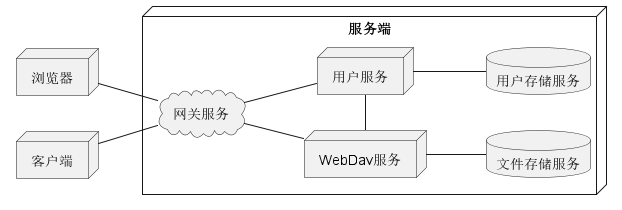
\includegraphics[scale=0.55]{examples/系统架构图.png}
    \caption{系统架构}
    \label{fig:sysarch}
\end{figure}

本系统的总体架构如图\ref{fig:sysarch}所示,浏览器或客户端可通过网关访端务端,网关会将请求转发给用户服务或WebDav服务。其中用户服务负责处理用户请求,如登录、注册等;而WebDav服务负责处理文件请求,如文件的上传、下载、移动、删除、预览等。

\subsection{模块设计}

本章节将描述云盘系统中的主要模块设计,包括用户服务模块和文件服务模块。

\subsubsection{用户服务模块}

用户服务模块包括用户服务和用户存储(数据库)服务,用户服务和用户存储服务之间通过内部网络通信。

\begin{figure}[H]
    \centering
    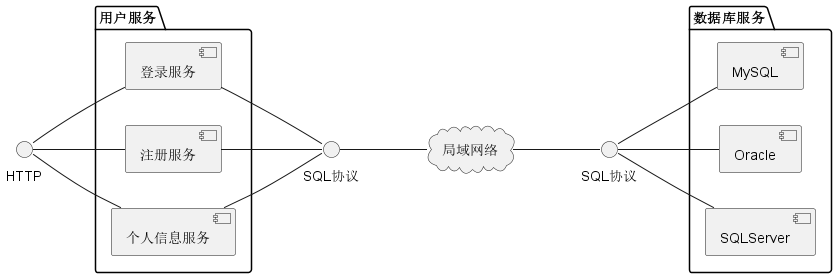
\includegraphics[scale=0.4]{examples/用户服务模块.png}
    \caption{用户服务模块}
    \label{fig:usersrv}
\end{figure}

如图\ref{fig:usersrv}所示,用户服务中包含登录、注册、个人信息处理等业务,用户服务通过HTTP协议接收请求,之后通过SQL协议和局域网络与数据库进行交互。

考虑到与数据库的交互需要适配不同类型的数据库,如MySQL、Oracle、SQLServer等,逻辑较为复杂,这里提出几种设计模式来抽象为该步骤,以便之后的实现。

\begin{figure}[H]
    \centering
    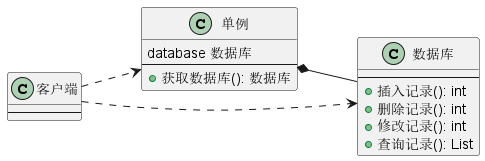
\includegraphics[scale=0.7]{examples/数据库服务-单例模式.png}
    \caption{基于单例模式的数据库服务实现}
    \label{fig:dbsrv_single}
\end{figure}

\begin{figure}[H]
    \centering
    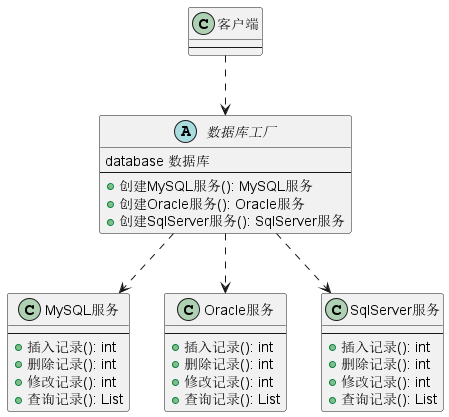
\includegraphics[scale=0.5]{examples/数据库服务-工厂模式.png}
    \caption{基于工厂模式的数据库服务实现}
    \label{fig:dbsrv_factory}
\end{figure}

\begin{figure}[H]
    \centering
    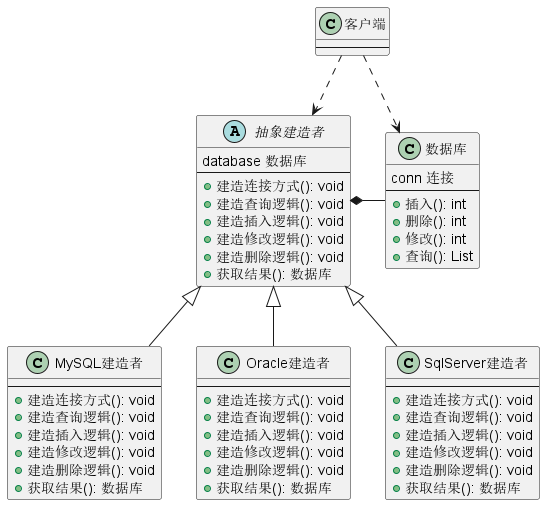
\includegraphics[scale=0.5]{examples/数据库服务-建造者模式.png}
    \caption{基于建造者模式的数据库服务实现}
    \label{fig:dbsrv_builder}
\end{figure}

这里提出了3种数据库服务的设计模式,如图\ref{fig:dbsrv_single},\ref{fig:dbsrv_factory},\ref{fig:dbsrv_builder}所示,分别为单例模式、工厂模式和建造者模式:
\begin{itemize}
    \item 单例模式。数据库服务仅为整个系统创建一个单例,保证所有线程使用相同的服务,避免不同线程造成冲突。
    \item 工厂模式。通过一个数据库工厂来创建基于不同数据库系统的数据库服务,保证该模块可以适配不同的数据库系统。
    \item 建造者模式。将数据库服务的创建逻辑分解为多个步骤,以简化操作。
\end{itemize}

事实上,在代码实现时,可以采用多个设计模式的混合策略。如工厂中的每个创建方法都采用建造者模式逐步构建;其次可以引入单例模式,如果服务已经被创建,就返回现有服务而不要创建新的服务。

\subsubsection{文件服务模块}

文件服务模块包括WebDav服务和文件存储服务,其中文件存储可以是本地的文件系统,也可以是远程的文件系统。

\begin{figure}[H]
    \centering
    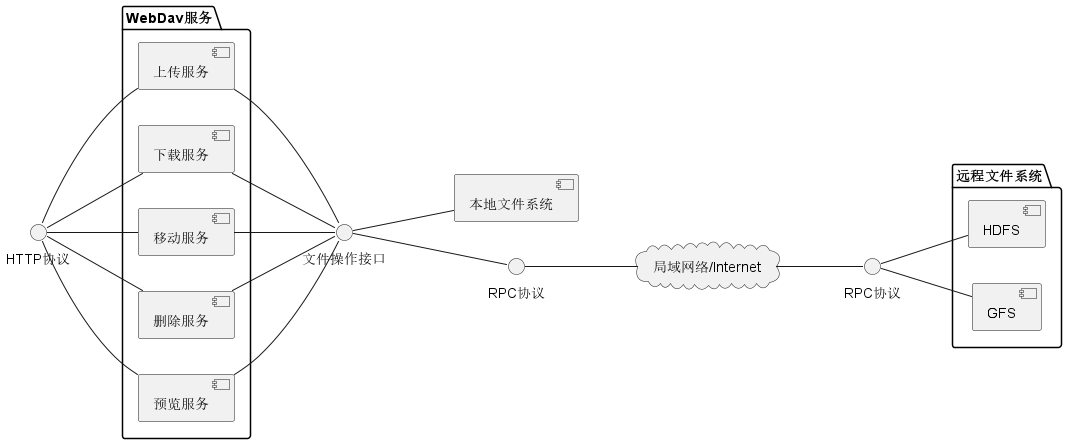
\includegraphics[scale=0.3]{examples/文件服务模块.png}
    \caption{文件服务模块}
    \label{fig:filesrv}
\end{figure}

文件服务模块的架构如图\ref{fig:filesrv}所示,用户请求通过HTTP协议发送给WebDav服务,WebDav处理文件的上传、下载、删除、移动、预览等请求,并于文件系统进行交互。

考虑到该模块需要支持不同的文件系统,本系统进行了高度的抽象,将本地/远程的文件系统交互抽象为一个接口,在此基础上实现本地文件系统的交互逻辑和基于RPC协议的远程文件系统交互逻辑。该部分同样可以采用单例、工厂、建造者等设计模式,与上一部分大致相同。